\documentclass[conference]{IEEEtran}
\usepackage[table]{xcolor}
\usepackage{tabularx}
\usepackage{graphicx}
\usepackage{amsmath}
\usepackage{listings}
\lstset{frame=single, language=python, tabsize=4}
\usepackage{tikz}
\usetikzlibrary{arrows.meta,automata,quotes,positioning,babel}
\usetikzlibrary{shapes.geometric, arrows}


\begin{document}
	\title{Deep Learning Approach to Link Weight Prediction}
	\author{
		\IEEEauthorblockN{Yuchen Hou}
		\IEEEauthorblockA{
			School of Electrical Engineering and Computer Science \\
			Washington State University, Pullman, WA 99164 \\
			yuchen.hou@wsu.edu
		}
		\and
		\IEEEauthorblockN{Lawrence B. Holder}
		\IEEEauthorblockA{
			School of Electrical Engineering and Computer Science \\
			Washington State University, Pullman, WA 99164 \\
			holder@wsu.edu
		}
	}
	\maketitle

\begin{abstract}
	Deep learning has been successful in various domains 
	including image recognition, speech recognition and natural language 
	processing.
	However, the research on its application in graph mining is 
	still in an early stage.
	Here we present Model R, a neural network model created to provide a deep 
	learning approach to link weight prediction problem.
	This model extracts knowledge of nodes from known links' weights and 
	uses this knowledge to predict unknown links' weights.
	We demonstrate the power of Model R through experiments and compare it with 
	stochastic block model and its derivatives.
	Model R shows that deep learning can be successfully applied to 
	link weight prediction and it outperforms stochastic block model and its derivatives by up to 73\% in terms of prediction accuracy.
	We anticipate this new approach to provide effective solutions to more
	graph mining tasks.
\end{abstract}

\section{Introduction}
Both academia and industry have seen pervasive adoption of deep learning 
techniques powered by neural network models since early 2010s,
when they began to outperform other machine learning techniques in various 
application domains, e.g.,
speech recognition \cite{hannun2014deep},
image recognition \cite{simonyan2014very},
natural language processing \cite{yao2013recurrent},
recommendation systems \cite{barkan2016item2vec},
and graph mining \cite{grovernode2vec}.
These neural net models can not only achieve higher prediction accuracy than 
traditional models,
but also require much less domain knowledge and engineering.

Among those domains,
graph mining is a new and active application area for deep learning.
The research in graph mining has advanced many fields
where objects and their relations can be modeled by nodes and links in a network, e.g.,
computer networks \cite{bermond1995distributed},
social networks \cite{cook2006mining},
protein interaction networks \cite{bader2003automated},
ecological food webs \cite{brown2003ecological},
and citation networks \cite{greenberg2009citation}.
An important task in graph mining is link prediction \cite{liben2007link} 
\cite{al2006link},
e.g., to predict whether a person will follow another person in a social network.
To be more specific,
the link prediction problem actually refers to link existence prediction:
to predict whether a link from a node to another node exists or will form.
Link existence prediction is a well-known problem,
but one of its related problems is not: link weight prediction.
Link weight prediction is to predict the weight of a link,
i.e., to predict how likely or how strong two nodes are connected.
Link weight prediction is more informative in many scenarios.
For example, when describing the connection of two users in a social network,
a description "Alice texts Bob 128 times per day" is more informative than
"Alice likes Bob" .
A special case of link weight prediction is collaborative filtering.
For example, to predict users' ratings to movies
is to predict the link weights on the bipartite graph
where the two disjoint node sets are users and movies.

As neural nets have demonstrated their power in many domains,
we naturally wonder if we can apply them in prediction tasks in graph mining,
and what kind of techniques are helpful in using their power.
We want to create a technique to predict link weights in a graph using a 
neural net model.
The estimator should learn to represent the graph in a meaningful way and to 
learn to predict the target link weights using the representation it learns.
The contribution of this paper is
a deep learning approach to link weight prediction problem.

\section{Problem}
We consider the problem of link weight prediction in a weighted directed graph.
We first take a look at an example of the problem,
and then give the problem a definition.
An undirected graph can be reduced to a directed graph by converting each weighted undirected link to two directed links with the same weight and opposite directions,
so the prediction for a weighted undirected graph is a special case of the problem we consider.

\subsection{Problem example}
Let us look at an example of link weight prediction - message volume prediction in a social network, shown in Figure \ref{fig:example} and Table \ref{tab:example}.
In this example, there are 3 users in a social network: A, B and C.
Each user can send any amount of text messages to every other user.
We know the message size transmitted between A and C, B and C, but not A and B.
We want to predict the message size transmitted between A and B.
\begin{figure}[!htb]\centering
	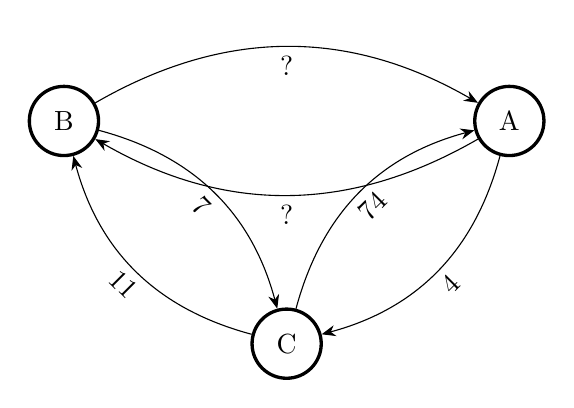
\begin{tikzpicture}[
	node distance = 4cm,
	on grid,
	> = {Stealth[length=5pt,width=4pt]},
	every state/.style = {very thick},
	every edge quotes/.style = {sloped, anchor=north}
	]
	\node[state] (B) {B};
	\node[state] (C) [below right=of B] {C};
	\node[state] (A) [above right=of C] {A};
	\path[->]   
	(A) edge[bend left,"?"]   (B)
	(B) edge[bend left,"7"]   (C)
	(B) edge[bend left,"?"]   (A)
	(A) edge[bend left,"4"]   (C)
	(C) edge[bend left,"74"]  (A)
	(C) edge[bend left,"11"]  (B);
	\end{tikzpicture}
	\caption{
		An example of link weight prediction in a weighted directed graph -
		message volume prediction in a social network.
		There are 3 users - A, B and C - in this network.
		Each user can send any amount of text messages to every other user.
		Here is what we know:
		A sent 4 messages to C,
		B sent 7 messages to C,
		and C sent 74 and 11 messages to A and B.
		What we do not know and what we want to predict is
		the message volume A and B sent to each other.
		}
	\label{fig:example}
\end{figure}
\begin{table}[!htb]\centering
	\caption{
		The same example as Figure \ref{fig:example}, but with edge list representation for the network.
	}
	\begin{tabularx}{0.45\textwidth}{|X|X|c|}  \hline \rowcolor{blue!40}
		Source node & Destination node & Link weight \\ \hline
		A & B & ? \\ \hline
		A & C & 74 \\ \hline
		B & A & ? \\ \hline
		B & C & 7 \\ \hline
		C & A & 4 \\ \hline
		C & B & 11 \\ \hline
	\end{tabularx}
	\label{tab:example}
\end{table}
This is a simplified network similar to many real social networks, where every user interacts with other users by posting, sharing, following or liking them.
There can not be any logical approach to derive the unknown message volumes,
as they have randomness.
But there can be statistical approaches to build models to predict them.
The ability to predict these interactions potentially allows us to recommend new connections to users:
if A is predicted/expected to send a large amount of messages to B by some model,
and A is not connected to B yet,
we can recommend B as a new connection to A.

\subsection{Problem definition}
Now we define the link weight prediction problem in a weighted directed graph.
\begin{itemize}
	\item Given a weighted directed graph with the node set V and link subset E
	\item Build a model w = f(x, y) where x and y are nodes and w is the weight of link (x, y) that can predict the weight of any link
\end{itemize}
For every possible link (1 out of $ n^2 $, where n is the number of nodes), 
if we know its weight, we know it exists;
if we do not know its weight, we do not know it exists.
This is a very practical point when we handle streaming graphs:
for any possible link,
we either know it exists and know its weight (if it has been streamed in), or we do not know if the link will ever exist, nor know its weight.

\section{Existing approaches}
In our literature study on previous research in the link weight prediction problem,
we have found few existing approaches and no deep learning ones.
In this section,
we review these existing approaches.

\subsection{Node similarity model}
This approach is designed for undirected graphs.
It assumes the weight of a link between two nodes 
is proportional to the similarity of those two nodes.
It employs a linear regression model \cite{zhao2015prediction}:
\begin{align*}
	w_{xy} = k \cdot s_{xy}
\end{align*}
where k is the regression coefficient,
$ w_{xy} $ is the weight of the link between node x and node y,
and $ s_{xy} $ is the similarity of x and y, calculated based on their common neighbors:
\begin{align*}
	s_{xy} = \sum_{z \in N(x) \cap N(y)} F
\end{align*}
where N(x) is the set of neighbors of node x, z is any common neighbor of x and y,
and F is an index factor which has nine different forms, shown in Table \ref{tab:indexes}.
\begin{table}[!htb]\centering
	\caption{9 different forms of index factor F.}
	\begin{tabularx}{0.45\textwidth}{|>{\columncolor{blue!40}}X|X|X|X|}  \hline \rowcolor{blue!40}
		& Common Neighbors & Adamic-Adar & Resource Allocation \\ \hline
		Unweighted &
		\[1\] &
		\[\frac{1}{\log(d_z)}\] &
		\[\frac{1}{d_z}\] \\ \hline
		Weighted &
		\[w_{xz} + w_{zy}\] &
		\[\frac{w_{xz} + w_{zy}}{\log(1 + s_z)}\] &
		\[\frac{w_{xz} + w_{zy}}{s_z}\] \\ \hline
		Reliable-route Weighted &
		\[ w_{xz} \cdot w_{zy}\] &
		\[\frac{w_{xz} \cdot w_{zy}}{\log(1 + s_z)}\] &
		\[\frac{w_{xz} \cdot w_{zy}}{s_z}\] \\ \hline
	\end{tabularx}
	\label{tab:indexes}
\end{table}
In Table \ref{tab:indexes}, $ d_z $ is the degree of node z and $ s_z $ is the strength of node z:
\begin{align*}
s_z = \sum_{u \in N(z)} w_{zu}
\end{align*}
These nine forms represent three groups of measures of 2-hop paths connecting those two nodes:
\begin{itemize}
	\item Unweighted group \cite{adamic2003friends}: based on path existence - ignoring path weights
	\item Weighted group \cite{murata2007link}: based on path lengths - sum of path weights
	\item Reliable route weighted group \cite{taha1982operations}: based on path reliability - product of weights
\end{itemize}
And each group contains three forms:
\begin{itemize}
	\item Common Neighbors: pure path based
	\item Adamic-Adar: similar to Common Neighbors
	but depresses the contribution of common neighbors with high degree or high strength
	\item Resource Allocation: similar to Adamic-Adar but depresses more
\end{itemize}

\subsection{SBM (Stochastic Block Model)}
This approach is designed for unweighted graphs and uses only link existence information \cite{holland1983stochastic}.
The main idea is to partition nodes into L groups and connect groups with bundles.
In this way, the graph has a 2-level structure:
\begin{itemize}
	\item Lower level: each group consists of nodes which were topologically similar in the original graph
	\item Upper level: groups are connected by bundles
	to represent the original graph
\end{itemize}
Given a graph with adjacency matrix A, the SBM has the following parameters:
\begin{itemize}
	\item A: link existence matrix, where $ A_{ij} \in \{0, 1\} $
	\item z: the group vector,
	where $ z_i \in \{ 1 ... L \} $ is the group label of node i
	\item $ \theta $: the bundle existence probability matrix,
	where $ \theta_{z_i z_j} $ is the existence probability of bundle ($z_i, z_j$)
\end{itemize}
So the existence of link (i, j) $ A_{ij} $ is a binary random variable following the Bernoulli distribution:
\begin{align*}
	A_{ij} \sim B(1, \theta_{z_i z_j})
\end{align*}
The SBM fits parameters z and $ \theta $
to maximize the probability of observation A:
\begin{align*}
	P(A|z, \theta) 
	= \prod_{ij} \theta_{z_i z_j}^{A_{ij}}(1-\theta_{z_i z_j})^{1-A_{ij}}
\end{align*}
which we rewrite as log likelihood of observation A:
\begin{align*}
	&\log(P(A|z, \theta))\\
	=& \sum_{ij} (
	{A_{ij}} \log (\theta_{z_i z_j})
	+ (1 - {A_{ij}}) \log(1-\theta_{z_i z_j})
	)\\
	=& \sum_{ij} (
	{A_{ij}} \log (\frac{\theta_{z_i z_j}}{1-\theta_{z_i z_j}})
	+ \log(1-\theta_{z_i z_j})
	)
\end{align*}
which we rewrite as an exponential family:
\begin{align*}
	\log(P(A|z, \theta))
	= \sum_{ij} (
	T(A_{ij}) \eta(\theta_{z_i z_j})
	)
\end{align*}
where
\begin{align*}
	T(A_{ij}) = (A_{ij}, 1)
\end{align*}
is the vector-valued function of sufficient statistics of the Bernoulli random variable and
\begin{align*}
\eta(\theta) = ( \log(\frac{\theta}{1-\theta}), \log(1-\theta) )
\end{align*}
is the vector-valued function of natural parameters of the Bernoulli random variable.

\subsection{pWSBM (pure Weighted Stochastic Block Model)}
The pWSBM is designed for weighted graphs and uses only link weight information \cite{aicher2014learning}.
So it differs from SBM in a few ways described below.
Here we choose model link weight with normal distribution.
Adjacency matrix A becomes the link weight matrix:
\begin{align*}
	A_{ij} \in R
\end{align*}
$ \theta_{z_i z_j} $ becomes the weight distribution parameter of bundle ($z_i, z_j$):
\begin{align*}
	\theta_{z_i z_j} = (\mu_{z_i z_j}, \sigma_{z_i z_j}^2)
\end{align*}
$ T(A_{ij}) $ becomes the vector-valued function of sufficient statistics of the normal random variable:
\begin{align*}
	T(A_{ij}) = (A_{ij}, A_{ij}^2, 1)
\end{align*}
$ \eta(\theta) $ becomes the vector-valued function of natural parameters of the normal random variable:
\begin{align*}
	\eta(\theta)
	&= \eta(\mu, \sigma^2)\\
	&= (\frac{\mu}{\sigma^2}, -\frac{1}{2\sigma^2}, -\frac{\mu^2}{2\sigma^2})
\end{align*}
So the weight of link (i, j)  $ A_{ij} $ is a real random variable following the normal distribution:
\begin{align*}
	A_{ij} \sim N(\mu_{z_i z_j}, \sigma_{z_i z_j}^2)
\end{align*}
The pWSBM fits parameter z and $ \theta $
to maximize the log likelihood of observation A:
\begin{align*}
\log(P(A|z, \theta))
&= \log(P(A|z, \mu, \sigma^2))\\
&= \sum_{ij} (
A_{ij} \frac{\mu_{z_i z_j}}{\sigma_{z_i z_j}^2}
- A_{ij}^2 \frac{1}{2\sigma_{z_i z_j}^2}
- \frac{\mu_{z_i z_j}^2}{\sigma_{z_i z_j}^2}
)
\end{align*}

\subsection{bWSBM (balanced Weighted Stochastic Block Model)}
The bWSBM is a hybrid of SBM and pWSBM
and uses both link existence information and link weight information \cite{aicher2014learning}.
The hybrid log likelihood becomes:
\begin{align*}
&\log(P(A|z, \theta))\\
=& \alpha \sum_{ij \in E} (T_e(A_{ij}) \eta_e(\theta_{z_i z_j}))\\
& + (1 - \alpha) \sum_{ij \in W} (T_w(A_{ij}) \eta_w(\theta_{z_i z_j}))
\end{align*}
where pair $ (T_e, \eta_e) $ denotes the family of link existence distributions:
\begin{align*}
T_e(A_{ij}) &= (A_{ij}, 1)\\
\eta_e(\theta) &= ( \log(\frac{\theta}{1-\theta}), \log(1-\theta) )
\end{align*}
and pair $ (T_w, \eta_w) $ denotes the family of the link weight distributions:

\begin{align*}
T_w(A_{ij}) &= (A_{ij}, A_{ij}^2, 1)\\
\eta_w(\theta)
&= (\frac{\mu}{\sigma^2}, -\frac{1}{2\sigma^2}, -\frac{\mu^2}{2\sigma^2})
\end{align*}
and $ \alpha \in [0, 1]$ is a tuning parameter that determines their relative importance,
E is the set of observed interactions,
and W is the set of weighted edges.
In the following, we use $ \alpha = 0.5 $ following the practice in \cite{aicher2014learning}.

\subsection{DCWBM (Degree Corrected Weighted Stochastic Block Model)}
The DCWBM is designed to incorporate node degree
by replacing pair $ (T_e, \eta_e) $ in the bWSBM with:
\begin{align*}
	T_e(A_{ij}) &= (A_{ij}, -d_id_j)\\
	\eta_e(\theta) &= (\log\theta, \theta)
\end{align*}
where $ d_i $ is the degree of node i \cite{aicher2014learning}.

\subsection{Deep learning approaches to other related problems}
There are a few deep learning approaches to
the node classification problem (i.e., to predict whether a node has a label) and 
link existence prediction problem (i.e., to predict whether a link exists).
Two earlier approaches are graph neural nets and relational neural 
nets \cite{scarselli2009graph},
where neural nets are incorporated into a traditional iterative graph 
information propagation approach.
A newer approach is deep walk \cite{perozzi2014deepwalk}, 
where a graph is reduced to a natural language corpus so that existing neural 
net model designed for natural language processing - skip-gram model - can handle the graph.
A very recent approach is node2vec \cite{grovernode2vec},
which uses the same skip-gram model, 
but a different way to reduce the graph to a natural language corpus.

\section{Observations}
As deep learning techniques become more powerful and standardized,
a key process of a domain-specific deep learning application
is to represent entities as vectors,
because a neural net needs vectors as inputs.
In this section, we make some observations about this process,
which lead to the deep learning approach to link weight prediction.

\subsection{Entities and representations}
First of all, we summarize how a neural net represents various types of 
entities in different domains with different relations, as shown in 
Table \ref{tab:domains}.
An image in image recognition is represented as
a 2D light amplitude array with dimensions height and width;
an audio/spectrogram in speech recognition is represented as
a 2D sound amplitude array with dimensions time and frequency.
The relation between two images or two audio is not commonly used. 
Words in natural languages, items in recommendation systems, and nodes 
in graphs can be represented by vectors (1D numeric arrays).
The	relations between two words, two items and two nodes are commonly 
used to learn these vectors.
It is clear that representations for all the entities are numeric arrays, 
because neural nets rely on neurons' activations and communications, which 
are both numeric.
\begin{table*}[!htb]
	\centering
	\caption{
		A summary of various types of entities, their numeric
		representations and inter-entity relations in different domains.
	}
	\begin{tabularx}{1\textwidth}{|c|c|X|X|} \hline \rowcolor{blue!40}
		Domain & Entity & Relations & Representation \\ \hline
		image recognition & image & N/A & 2D light amplitude array[width, height] \\ \hline
		speech recognition & audio/spectrogram  & N/A & 2D sound amplitude array[time, frequency] \\ \hline
		natural language processing & word   & co-occurrences of words in a context & 1D array (i.e., word vector) \\ \hline
		recommendation systems & item   & co-purchases of items in a order & 1D array (i.e., item vector) \\ \hline
		graph mining & node   & connections of nods (i.e., links) & 1D array (i.e., node vector) \\ \hline
	\end{tabularx}
	\label{tab:domains}
\end{table*}

\subsection{Mapping entities to vectors}
The word2vec technique is famous for using a neural net to learn to map every 
entity (word in this case) in a vocabulary to a vector without any domain 
knowledge \cite{mikolov2013efficient}.
The subsequent techniques item2vec \cite{barkan2016item2vec}
and node2vec \cite{grovernode2vec} use the same skip-gram 
model used in word2vec to map items and nodes to vectors.
In a corpus, every word is described/defined only by related words in its 
contexts, by implicit relations between words in word co-occurrences.
Nonetheless, the neural net can learn from word co-occurrences and map words to 
vectors accordingly,
such that the relations between words are preserved in the word vector space 
\cite{mikolov2013distributed}.
The same arguments apply to relations between items and between nodes.

\subsection{Mapping nodes to vectors}
The relation between nodes is quite different from that between words:
\begin{itemize}
	\item The weight of a link from one node to another specifically tells us
	how strong one node connects to the other;
	this type of relation has regular and explicit form:
	entity - relation - entity.
	\item On the other hand, the co-occurrences of words 
	(e.g., in the context [The quick brown fox jumps over the lazy dog])
	implicitly tell us these words are related
	but do not tell us any specific relations
	(e.g., Are [quick] and [brown] related? What is the relation between [fox] and [jumps]? Is [over] a relation or entity?).
\end{itemize}
Natural languages do not have the notion that
all information can be described as entities and their relations, as in graphs.
For a neural net, 
words can simply show up in sequences from day-to-day conversations,
in many flexible and unpredictable ways, with little structure or regularity.
Therefore, the skip-gram model, designed to handle natural languages,
can not take advantage of highly structured data in graphs.
This suggests that a neural net, if correctly designed to handle graphs,
should be able to learn a node-to-vector mapping supervised by the link weight,
in a more specific, direct and simply way than it learns word-to-vector 
mappings supervised by word co-occurrences.

\section{Approach}
Following the above observations,
we build an estimator with a neural net model using a node pair as its input
and the weight of the link connecting the nodes as its output.

\subsection{Model R}
We design the model in the estimator as a fully connected neural net which we call Model R (R as in relation), shown in Figure \ref{fig:model}.
We have considered a convolutional neural net as an alternative,
but we decided it would not be a good fit for this application.
These node vectors do not any spacial property
for a convolutional neural network to take advantage of,
compared to the 2D array of an image where the spacial location of each pixel
has significant meaning (e.g., relative distances of pixels).
These node vectors do not have any of those invariance properties in image either,
such as translation invariance, rotation invariance,
size invariance and illumination invariance.

\begin{figure*}[!htb]
	\centering
	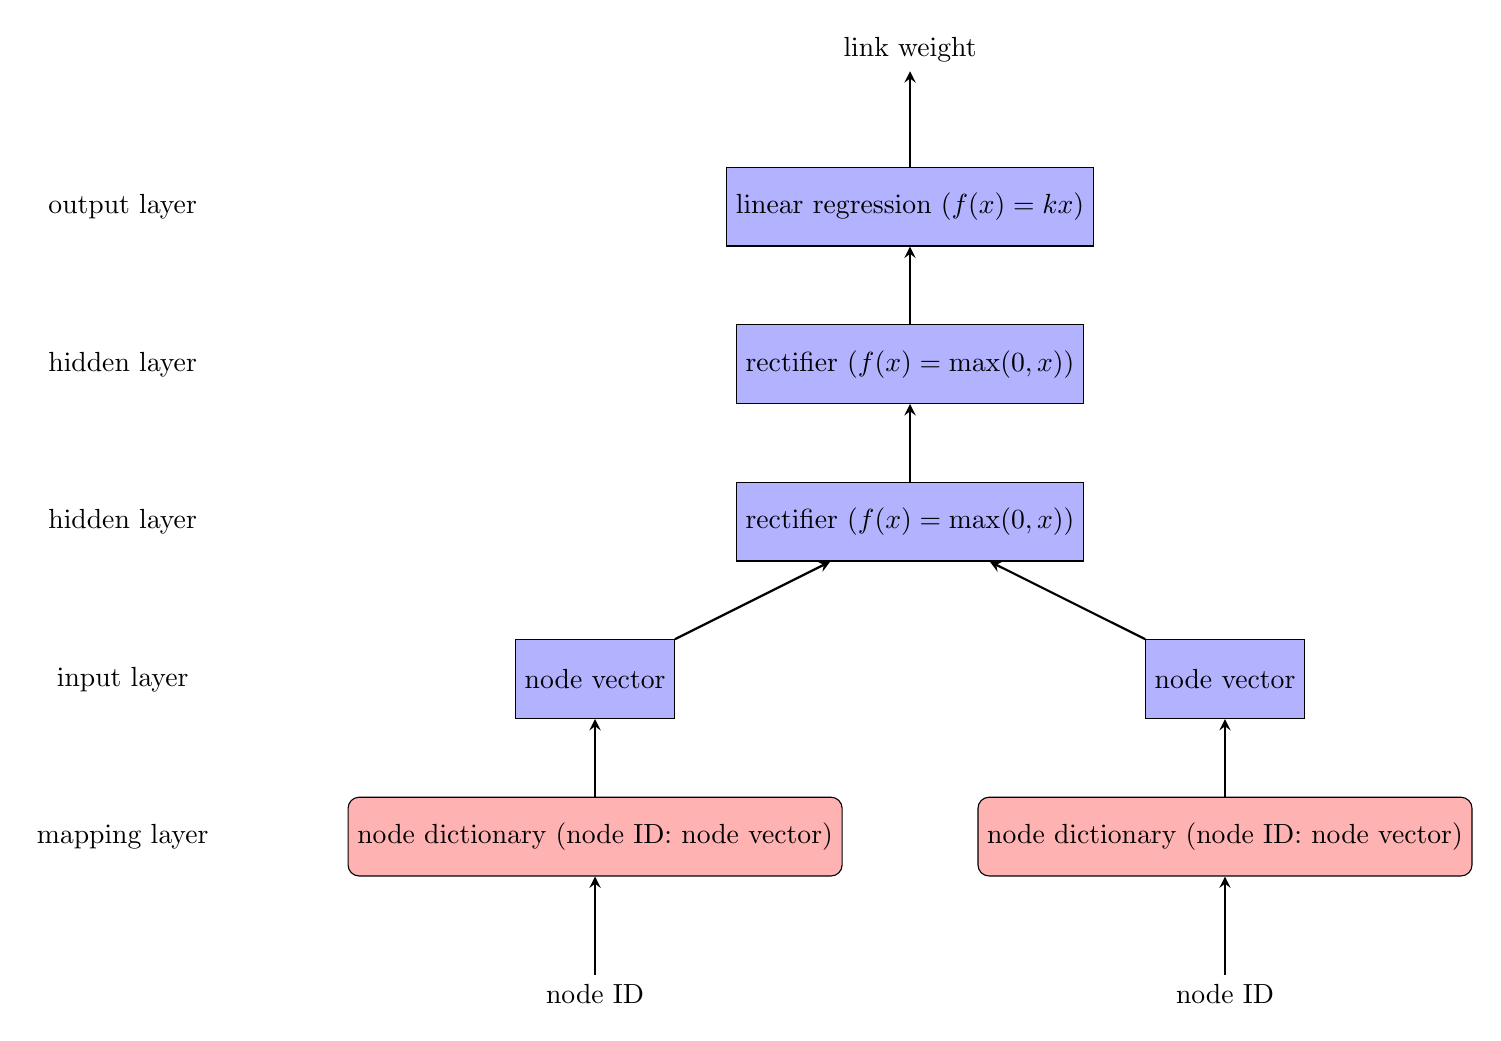
\begin{tikzpicture}[node distance=2cm]
	\tikzstyle{startstop} = [rectangle, rounded corners, minimum width=1cm, 
	minimum height=1cm, text centered, draw=black, fill=red!30]
	\tikzstyle{process} = [rectangle, minimum width=1cm, minimum height=1cm, 
	text centered, draw=black, fill=blue!30]
	\tikzstyle{arrow} = [thick,->,>=stealth]
	\node (linearRegression) [process] {linear regression ($ f(x) = kx $)};
	\node (relu0) [process, below of=linearRegression] {rectifier ($ f(x) = \max (0, x) $)};
	\node (relu) [process, below of=relu0] {rectifier ($ f(x) = \max (0, x) $)};
	\node (linear1) [process, below of=relu, xshift=-4cm] {node vector};
	\node (linear2) [process, below of=relu, xshift=4cm] {node vector};
	\node (oneHot1) [startstop, below of=linear1] {node dictionary (node ID: node vector)};
	\node (oneHot2) [startstop, below of=linear2] {node dictionary (node ID: node vector)};
	\node (weight) [above of=linearRegression] {link weight};
	\node (output) [left of=linearRegression, xshift=-8cm] {output layer};
	\node (hidden0) [below of=output] {hidden layer};
	\node (hidden) [below of=hidden0] {hidden layer};
	\node (input) [below of=hidden] {input layer};
	\node (mapping) [below of=input] {mapping layer};
	\node (source) [below of=oneHot1] {node ID};
	\node (destination) [below of=oneHot2] {node ID};
	\draw [arrow] (source) -- (oneHot1);
	\draw [arrow] (destination) -- (oneHot2);
	\draw [arrow] (oneHot1) -- (linear1);
	\draw [arrow] (oneHot2) -- (linear2);
	\draw [arrow] (linear1) -- (relu);
	\draw [arrow] (linear2) -- (relu);
	\draw [arrow] (relu0) -- (linearRegression);
	\draw [arrow] (relu) -- (relu0);
	\draw [arrow] (linearRegression) -- (weight);
	\end{tikzpicture}
	\caption{
		Model R for a weighted graph.
		Only layers and their connections are shown,
		while the units in each layer and their connections are not shown.
		We feed every node to the estimator by feeding the ID.
		During learning,
		the estimator learns and populates the vectors in the tables.
	}
	\label{fig:model}
\end{figure*}
The model contains the following layers:
\begin{itemize}
	\item A mapping layer that maps node IDs to node vectors.
	In the node dictionary,	the key is the node ID, the value is the node vector,
	which is learned through back propagation and stochastic gradient descent.
	\item An input layer directly activated by the node dictionaries.
	Its activations are the two node vectors.
	\item Multiple fully connected hidden layers of rectified linear units
	(only two layers are shown in the figure).
	These units employ the rectifier ($ f(x) = \max (0, x) $)
	as their activation function.
	These layers learn to extract more and more abstract weight-relevant 
	information.
	\item An output layer with a linear regression unit.
	This unit employs linear regression ($ f(x) = kx $) as its activation function.
	It learns to predict the link weight as a real number
	using abstracted weight-relevant information.
\end{itemize}
Link weights provide the information about nodes.
We fully take this property into account and design this model to learn 
complex and unobservable node information (i.e., node vectors) 
supervised by a simple and observable relations between nodes (i.e., link weight).

\subsection{Learning techniques}
The estimator uses the above model and a number of popular deep learning 
techniques:
\begin{itemize}
	\item Backpropagation: propagation of the error gradients from output layer 
	back to each earlier layer \cite{rumelhart1988learning}
	\item Stochastic gradient descent: the optimization that minimizes 
	the error (descending against the error gradient in weight space) for a 
	random sample in each gradient descent step \cite{lecun2012efficient}
	\item Mini-batch: the modification to stochastic gradient descent to 
	accelerate and smooth the descent by minimizing the error for a small 
	random batch of samples in each gradient descent step \cite{mairal2010online}
	\item Early stopping: the regularization used to reduce over-fitting during the iterative learning process by stopping the learning when validation error stops decreasing \cite{smale2007learning}
\end{itemize}

\subsection{Model R design parameters}
Given the above design and learning techniques,
there are still a number of design parameters we can adjust,
e.g., the number of layers, the number of units in each layer,
and the activation function of each unit.
Now we briefly discuss different options for these parameters,
and also some justifications for our choices.
\begin{itemize}
	\item The choice of rectifier as the activation function is a relatively easy one.
	Compared to earlier popular activation functions like sigmoid function
	($ f(x) = (1 + \exp(-x))^{-1} $),
	rectifier not only simplifies and accelerates computation,
	but also eliminates vanishing gradient problems,
	and has become the most popular activation function
	for deep neural networks \cite{lecun2015deep}.
	\item The choice of layer size is related to
	the number of examples in the dataset.
	Naturally, the larger the dataset is,
	the more discriminative the model should be,
	and consequently higher degrees of freedom,
	higher dimensions of vectors and larger layer sizes.
	Empirically, we typically set the layer size as a logarithm function of the dataset size:
	\[d = log_2(n)\]
	where d (as in dimension) is the layer size and n is the dataset size.
	\item The choice of number of layers is related to the complexity of the relation between the input and the output of the model.
	As a trivial example, if the input and the output have linear relation,
	no hidden layer is necessary and the model is simply a linear model.
	If the input and the out put have non-linear relation,
	the more complex the relation is, the more number of layers are necessary.
	Empirically, we typically set the the layer size to 4,
	and occasionally down to 2 and up to 8.
\end{itemize}
We naturally assume the most optimum design parameters are dataset dependent.
However, we do not know any theoretical way to calculate the most optimum parameters based on the statistic signatures of a specific dataset.
Therefore, 
In this work, we evaluate different parameter choices through a few experiments.
We will work on design parameter optimization in our future research.

\section{Experiments}
We evaluate Model R experimentally with SBM, pWSBM, bWSBM and DCWBM as baselines,
and compare their prediction errors on several datasets.
We use the same datasets and experiment process used in a recent study of these baselines \cite{aicher2014learning}.
The results show 
that Model R can achieve much lower prediction error than the baseline models.

\subsection{Datasets}
The experiments use four datasets summarized in Table \ref{tab:datasets}.
\begin{table*}[!htb]\centering
	\caption{The datasets used in experiments.}
	\begin{tabularx}{\textwidth}{|c|c|c|c|X|}  \hline \rowcolor{blue!40}
		Dataset name & Node count & Node type & Link count & Link weight type \\ \hline
		Airport\cite{colizza2007reaction} & 500 & busiest airports in US & 5960 & number of passengers traveling from one airport to the other\\ \hline
		Collaboration\cite{pan2012world} & 226 & nations on Earth & 20616 & number of papers written by authors from the two nations \\ \hline
		Congress\cite{porter2005network} & 163  & 102nd US Congress committees & 26569 & interlock value of shared members from the two committees \\ \hline
		Forum\cite{opsahl2009clustering}  & 1899 & users of a student social network & 20291 & number of messages sent from one student to the other \\ \hline
	\end{tabularx}
	\label{tab:datasets}
\end{table*}

\subsection{Experiment process}
We do the same experiment for each dataset.
All the link weights are normalized to the range [-1, 1] after applying a logarithm function.
Each experiment consists of 25 independent trials.
In each trial, we split the dataset randomly into 3 subsets:
\begin{itemize}
	\item 70\% into training set
	\item 10\% into validation set
	\item 20\% into testing set
\end{itemize}
We use mean squared error as the prediction accuracy metric.
For each experiment, we report the mean and standard deviation of the errors from 25 trials.
The pseudo code of the experiment process is shown in Figure \ref{fig:code}.
\begin{figure*}[!htb]\centering
	\begin{lstlisting}
		def main():
			for dataset in [Airport, Collaboration, Congress, Forum]:
				(error_mean, error_standard_deviation) = do_experiment(dataset)
		def do_experiment(dataset):
			errors = list()
			for trial in range(25):
				testing_error = append(evaluate_model_on(dataset))
				errors.append(testing_error)
			return (errors.mean(), errors.standard_deviation())
		def evaluate_model_on(dataset):
			(training_set, validation_set, testing_set) = split(dataset)
			while validation_error decreases:
				training_error = estimator.learn(training_set)
				validation_error = estimator.predict(validation_set)
			testing_error = estimator.predict(testing_set)
			return testing_error
	\end{lstlisting}
	\caption{
		The pseudo code of the experiment process.
		The estimator.learn() method learns for one epoch through the training set, updating the weights after each example batch.
	}
	\label{fig:code}
\end{figure*}

\subsection{Experiment results}
In our experiments,
Model R's error is lower than every other model on every dataset,
shown in Figure \ref{fig:errors}.
\begin{figure*}[!htb]\centering
	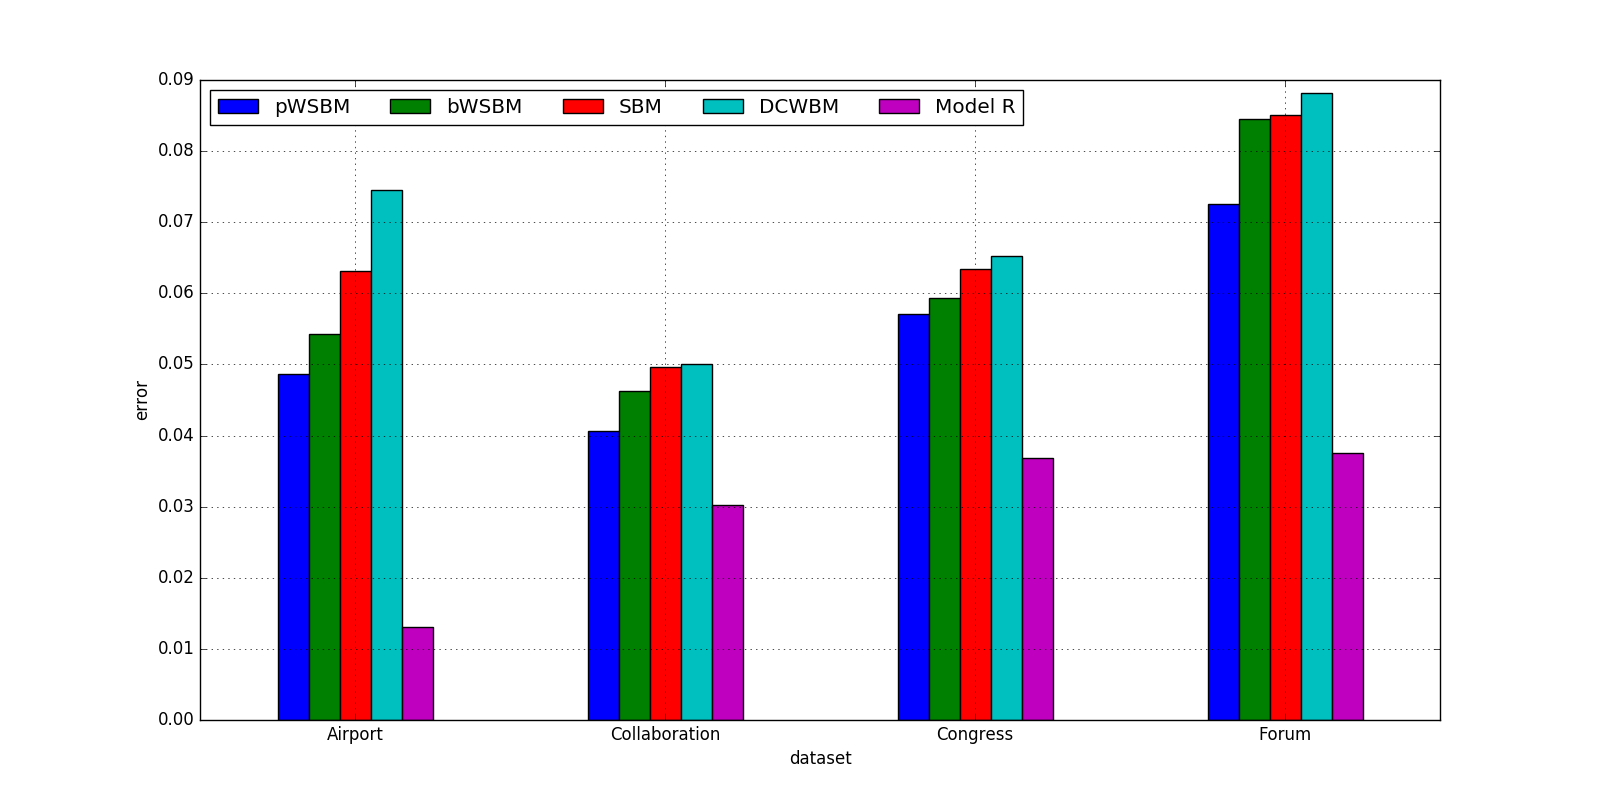
\includegraphics[width=1\textwidth]{link-weight-errors}
	\caption{
		The mean squared errors of 5 models on 4 datasets:
		Model R has lower error than every other model on every dataset.
		Every error value shown here is the mean errors for the 25 trials in the experiment.
	}
	\label{fig:errors}
\end{figure*}
In this section we compare Model R with the baseline models on every dataset.
Given the dataset,
we regard ModelRError (as well as BaselineError) as a random variable
so each trial generates an example of it.
We can do a t-test to justify the significance of difference between the means of variables ModelRError and BaselineError.
The mean of a variable is not the same as the mean of a sample of the variable.
More specifically, a variable can generate two samples with different sample means,
therefore two samples with different means do not imply the two variables generating them have different means.
For each dataset, we do a t-test for the two variables where the null hypothesis is that the two variables have the same mean:
\begin{align*}
\overline{X_1} == \overline{X_2}
\end{align*}
where $ X_1 $ and $ X_2 $ are ModelRError and BaselineError and
where $ \overline{X} $ is the mean of variable X.
The standard deviation $ s $ of variable X is defined as:
\begin{align*}
	s_i &= \sqrt{\overline{(X_i - \overline{X_i})^2}}
\end{align*}
Welch's t-test defines its statistic t and degrees of freedom v as:
\begin{align*}
	t &= \frac{
		\overline{X_1} - \overline{X_2}
		}{
		\sqrt{\frac{s^2_1}{N_1} + \frac{s^2_2}{N_2}}
		}\\
	v &= \frac{
		(\frac{s^2_1}{N_1} + \frac{s^2_2}{N_2})^2
		}{
		\frac{s^4_1}{N_1^2(N_1-1)} + \frac{s^4_2}{N_2^2(N_2-1)}
		}
\end{align*}
where $ N_i $ is the sample size of variable $ X_i $.
The Student's t-distribution defines its probability density function f(x) as:
\begin{align*}
f(x) = \frac{\Gamma(\frac{v+1}{2})}{\sqrt{v\pi}\Gamma(\frac{v}{2})}
((1+\frac{x^2}{v})^{-\frac{v+1}{2}})
\end{align*}
Welch's t-test defines its p value as the Student's t-distribution cumulative density function:
\begin{align*}
p = 2 \int_{-\infty}^{-|t|} f(x) dx
\end{align*}
The smaller p is, the more confidently we can reject the null hypothesis, i.e., accept that:
\begin{align*}
\overline{ModelRError} \neq \overline{BaselineError}
\end{align*}
Typically there is a domain specific threshold for p, e.g., 0.1 or 0.01. If p is smaller than the threshold we reject the null hypothesis.
We calculate the p value and also error reduction from baseline to Model R as:
\begin{align*}
Reduction = \frac{BaselineError - ModelRError}{BaselineError}
\end{align*}
The p value is almost 0 for all datasets and error reduction is significant,
shown in Table \ref{tab:errors}.
Model R has lower error than every other model on every dataset,
reducing error by 25\% to 73\% from the best baseline model - pWSBM.
The number in every parenthesis is the standard deviation of the errors in 25 trials in the last digit. The very low p values strongly indicate the error reduction is significant.
\begin{table*}[!htb]\centering
	\caption{
		The mean squared errors with standard deviations of 5 models on 4 datasets.
	}
	\begin{tabularx}{\textwidth}{|c|X|X|X|X|X|c|c|} \hline \rowcolor{blue!40}
		Dataset & pWSBM & bWSBM & SBM & DCWBM & Model R & Reduction & p \\ \hline
		Airport & 0.0486 $ \pm $ 0.0006 & 0.0543 $ \pm $ 0.0005 & 0.0632 $ \pm $ 0.0008 & 0.0746 $ \pm $ 0.0009 & 0.013 $ \pm $ 0.001 & 73\% & 4.2e-66 \\ \hline
		Collaboration & 0.0407 $ \pm $ 0.0001 & 0.0462 $ \pm $ 0.0001 & 0.0497 $ \pm $ 0.0003 & 0.0500 $ \pm $ 0.0002 & 0.030 $ \pm $ 0.001 & 25\% & 9.1e-44 \\ \hline
		Congress & 0.0571 $ \pm $ 0.0004 & 0.0594 $ \pm $ 0.0004 & 0.0634 $ \pm $ 0.0006 & 0.0653 $ \pm $ 0.0004 & 0.036 $ \pm $ 0.003 & 35\% & 7.1e-35 \\ \hline
		Forum & 0.0726 $ \pm $ 0.0003 & 0.0845 $ \pm $ 0.0003 & 0.0851 $ \pm $ 0.0004 & 0.0882 $ \pm $ 0.0004 & 0.037 $ \pm $ 0.001 & 48\% & 4.2e-68 \\ \hline
	\end{tabularx}
	\label{tab:errors}
\end{table*}
These results show that Model R outperforms pWSBM on all these datasets.

\subsection{Model robustness}
In our experiments, we have not observed any significant (more than 5\%)
prediction error increase or decrease when we change parameters around the values
we typically choose.
Overall, Model R has demonstrated very high level of model robustness.

\subsection{Reproducibility}
In order to ensure the reproducibility of the experiment,
we specify the implementation details in this section:
\begin{itemize}
	\item Programming language: Python 3
	\item Python implementation: CPython 3.5
	\item Deep learning package: TensorFlow \cite{abadi2016tensorflow}
	\item Operating system: Ubuntu 16.10 64-bit
	\item Computer make and model: Lenovo ThinkCentre M83
	\item Memory: 16 GB
	\item Processor: Intel Core i7-4770 CPU @ 3.40GHz $ \times $ 8
\end{itemize}
The program uses all 8 threads of the processor.
Each experiment takes about one hour to finish,
depending on the dataset and parameters in the learning algorithm.
The program is open-source under MIT license hosted on Github \footnote{https://github.com/yuchenhou/elephant}
so that anyone can use it without any restriction.

\section{Conclusion}
Model R shows that deep learning can be successfully applied to link weight prediction problem.
It effectively learns complex and unobservable node information (i.e., node vectors) from simple and observable relations between nodes (i.e., link weight),
and uses that information to predict unknown link weights.
We anticipate this new approach will provide effective solutions to more
graph mining tasks.

Compared to SBM based approaches, Model R is much more accurate.
A few possible reasons are:
\begin{itemize}
	\item Higher level of discrimination for nodes:
	SBM based approaches do not differentiate nodes within a same group,
	and assume the weights of all links connecting two nodes from two groups
	follow the same distribution;
	Model R does not assume that,
	but gives every node a unique description - the node vector - so that
	it can have a more accurate description for every single node.
	\item Higher level of model flexibility:
	SBM based approaches assume the weight of every link follows
	a normal distribution;
	Model R does not assume that, but takes advantage of high flexibility of
	layers of non-linear neural network units,
	so that it can model very complex weight distributions.
\end{itemize}

\section{Future work}
There are three aspects we would like to study in our future work on this model.
In this section, we briefly discuss these three aspects.

The first one is the mapping layer of Model R.
In the current model, the mapping layer contains two independent node dictionaries
to learn the node vectors.
During learning stage, these two dictionaries learn to map the nodes to two spaces:
\begin{itemize}
	\item The source node dictionary maps nodes to source node space.
	\item The destination node dictionary maps nodes to destination node space.
\end{itemize}
A more intuitive approach is to have every node mapped to
one and only one node vector in both dictionaries,
as in the word2vec technique.
However, will this more intuitive approach actually perform better?
Or does it depend on whether the graph is undirected or directed?
These are interesting questions we can study in the future.

The second one is to handle more complex graphs
and especially for social network applications.
In particular, we want to handle graphs with node attributes.
Users can have labels like nationality, and real attributes like age.
One feasible approach is to append one unit for each of these attributes to the node vector.

The third one is to handle large dynamic graphs.
A social network can have a large volume of links collected continuously by a
distributed system.
A potential approach is to deploy an estimator to each computing node of
the distributed system and analyze a link stream there,
and let these estimators exchange the knowledge periodically.

\section*{Acknowledgements}
This material is based upon work supported by the National Science Foundation under Grant No. 1646640.

\bibliographystyle{IEEEtran}
\bibliography{references}
\end{document}
